\documentclass[11pt]{article}
\usepackage[margin=1in]{geometry}
\usepackage{amsmath,amssymb}
\usepackage{graphicx}
\usepackage{booktabs}
\usepackage{array}
\usepackage[colorlinks=true,linkcolor=blue,citecolor=blue,urlcolor=blue]{hyperref}
\hypersetup{
  pdftitle={Pitch-Dependent Electron Confinement in Helical Magnetic Geometries},
  pdfauthor={Zachary Auerbach}
}

% Paper #2 of the EHR project (paper #1 is ehr-paper.tex). Every figure and every
% quoted number comes from paper/figures/pitch_figures.py, which reads the runs
% archived in paper/data/ and prints the values used here. Build with
% `tectonic paper/pitch-confinement.tex`; the PDF is build output, not committed.

\newcommand{\us}{\ensuremath{\mu}s}

% keep tables and figures beside their text instead of on sparse float-only pages
\renewcommand{\topfraction}{0.85}
\renewcommand{\bottomfraction}{0.6}
\renewcommand{\textfraction}{0.12}
\renewcommand{\floatpagefraction}{0.8}

\title{Pitch-Dependent Electron Confinement in Helical Magnetic Geometries}
\author{Zachary Auerbach\thanks{ORCID: \href{https://orcid.org/0009-0001-3046-9104}{0009-0001-3046-9104}}}
\date{Draft, September 10, 2026}

\begin{document}
\maketitle

\begin{abstract}
Tilting magnetic field lines lengthens the path a magnetized electron must travel to reach an end wall, which suggests field-line pitch as a tunable confinement parameter for low-temperature plasma sources. We test this idea with kinetic simulations of electrons in 10~mTorr argon in a cylinder threaded by divergence-free helical fields, scanning the wall pitch ratio $B_\theta(R)/B_z$ at fixed $|B(R)| = 100$~G. For test particles the effect is large and lawful: confinement rises $2.8\times$ between pitch ratios 0 and 3, and across five radial twist profiles the median confinement time scales as $\langle |B|/B_z\rangle^{\alpha}$, with $\alpha \approx 1$ without collisions and $\alpha = 1.2$--$1.4$ from 3 to 30~mTorr. An exponent fitted to one profile predicts a force-free Beltrami profile to within 2\%, and the entire gain comes from suppressed end losses. Once electrons generate their own electrostatic field, the gain does not survive. With frozen ions the potential well compresses it to $1.17\times$; with mobile ions it never exceeds $1.32\times$ and falls to $0.97\times$ as the exit-speed ion Hall parameter is raised through unity to 2.35; and in source-sustained steady state bulk confinement changes by only $+9\%$ and $+2\%$ on either side of ion magnetization. Pitch acts instead on the equilibrium: it lowers the confining potential by 11--12\% at nearly fixed confinement and reduces the core share of the electron inventory by 20\% below and 34\% above ion magnetization. The self-consistent results are obtained in a space-charge-limited regime ($R/\lambda_D \approx 3$--4) without RF heating, and we discuss what they do and do not imply for quasineutral discharges.
\end{abstract}

\section{Introduction}
\label{sec:intro}

Magnetized low-temperature plasma sources---helicon, electron-cyclotron-resonance, and magnetically enhanced inductive sources---confine electrons with static fields whose geometry is fixed by the coil set, predominantly axial in linear devices \cite{lieberman,chabert,chen2015}. In a finite-length magnetized column electrons are lost mainly along the field to the end plates, while cross-field transport is set by collisions \cite{curreli2014}. A standard result of boundary-plasma physics is that parallel losses scale with the connection length, the distance along a field line between wall contacts, which the field-line pitch controls \cite{stangeby}. A helical field in a linear device offers the same lever in a simpler setting: a field line with an azimuthal component $B_\theta$ travels $|B|/B_z$ times farther per unit axial distance than a purely axial one.

A companion concept paper \cite{auerbach2026} proposed a source in which this pitch is tuned through coil currents, and stated as its fourth prediction that scanning the pitch at constant $|B|$ and RF power should change the coupled power and the density profile. Two questions need answers before such an experiment is worth building. First, does the path-length argument produce a quantitative transport law, and does that law depend only on the pitch at the wall or also on how the twist is distributed in radius? Second, does the effect survive once the plasma generates its own electric field? In a discharge the electron and ion loss rates are tied together by charge balance \cite{lieberman,simon1955}, so the slower species may set the bulk loss rate whatever pitch does to the electrons.

This paper addresses both questions with a deliberately reduced kinetic model, built up one physical ingredient at a time. Its results are:
\begin{enumerate}
  \item a geometric transport law, $\tau \propto \langle |B|/B_z \rangle^{\alpha}$, in which the field geometry enters through a single seeding-averaged path factor and the exponent is set by parallel collisionality, tested across five radial twist profiles including an out-of-sample prediction for a force-free Beltrami field (Section~\ref{sec:testparticle});
  \item a mechanism decomposition showing that at 100~G the pitch effect is field-line geometry amplified by collisions, with no measurable contribution from particle drifts (Section~\ref{sec:mechanism});
  \item self-consistent electrostatic studies---frozen ions, mobile ions scanned across ion magnetization, and a source-sustained steady state---in which the bulk-confinement gain does not survive while the equilibrium potential and density structure respond to pitch (Section~\ref{sec:selfconsistent});
  \item an explicit account of which conclusions depend on the space-charge-limited regime of the self-consistent model and on the absence of RF heating (Section~\ref{sec:limitations}).
\end{enumerate}
The outcome is a negative result for pitch as a confinement parameter along the transport pathway, and a narrower positive result for pitch as a control on equilibrium structure.

\section{Model}
\label{sec:model}

\subsection{Chamber and helical fields}
\label{sec:fields}

The chamber is a cylinder of radius $R = 0.1$~m and length $L = 0.4$~m filled with argon at $T_{\mathrm{gas}} = 300$~K; at the baseline pressure of 10~mTorr the neutral density is $n_n = 3.2\times10^{20}$~m$^{-3}$. The radial wall and both end plates absorb every particle that reaches them. The static magnetic field is
\begin{equation}
\mathbf{B} = B_z(r)\,\hat{\mathbf{z}} + B_\theta(r)\,\hat{\boldsymbol{\theta}}, \qquad B_r = 0,
\label{eq:field}
\end{equation}
which is divergence-free for any radial profiles. The scan variable is the wall pitch ratio
\begin{equation}
\Theta \equiv B_\theta(R)/B_z(R),
\end{equation}
and every field is normalized so that $|B(R)| = 100$~G at every $\Theta$. No field of the form~\eqref{eq:field} with tunable pitch has $|B|$ constant everywhere, so fixing the wall magnitude is the closest realization of the constant-$|B|$ scan proposed in Ref.~\cite{auerbach2026}. Two families of profiles are used:
\begin{itemize}
  \item \emph{Power law}: $B_z$ uniform and $B_\theta = \Theta B_z (r/R)^n$ with $n \in \{0.5, 1, 2, 4\}$. The case $n = 1$, uniform axial current density, is called the \emph{screw} field. Small $n$ places the twist in the core; large $n$ concentrates it at the wall.
  \item \emph{Beltrami}: $B_z = B_0 J_0(kr)$ and $B_\theta = B_0 J_1(kr)$, the force-free field with $\nabla\times\mathbf{B} = k\mathbf{B}$ \cite{taylor1974,freidberg}, with $k$ fixed by $J_1(kR)/J_0(kR) = \Theta$. Holding $|B(R)|$ fixed makes the on-axis field grow with pitch, to $1.66\,|B(R)|$ at $\Theta = 3$.
\end{itemize}

Field lines lie on cylinders of constant $r$, and $|B|$ is constant along each of them, so a collisionless electron feels no mirror force and keeps its parallel speed $v_\parallel$. Its axial speed is $v_\parallel B_z/|B|$, reduced by the local path factor
\begin{equation}
F(r) \equiv \frac{|B|}{B_z} = \sqrt{1 + \left(\frac{B_\theta}{B_z}\right)^2}.
\label{eq:pathfactor}
\end{equation}
Every profile reaches $F = \sqrt{1+\Theta^2}$ at the wall but distributes the twist differently inside it (Fig.~\ref{fig:law}a). The natural scalar measure of a field's geometry is therefore the path factor averaged over the region in which particles are seeded,
\begin{equation}
\langle F \rangle = \frac{\int_0^{0.9R} F(r)\, r\, dr}{\int_0^{0.9R} r\, dr},
\label{eq:meanF}
\end{equation}
listed at $\Theta = 3$ in Table~\ref{tab:scan}.

\subsection{Particles, collisions, and diagnostics}
\label{sec:particles}

Particles are advanced with the Boris algorithm \cite{boris1970,qin2013,birdsallLangdon} at $\omega_c\,\Delta t \le 0.2$, rising to 0.22 on the axis of the Beltrami field at the highest pitch. Collisions with the neutral background use test-particle Monte Carlo \cite{birdsall1991,vahedi1995}; the time step also satisfies $\nu_{\max}\,\Delta t \le 0.05$, so the collision probability $\nu(E)\,\Delta t$ is sampled directly at each step rather than through null collisions. Electrons undergo elastic scattering, isotropic with the exact fractional energy loss $(2m_e/M)(1-\cos\chi)$, and ionization, in which the 15.76~eV threshold is subtracted and the secondary electron is not tracked. The electron cross sections are log--log tables that reproduce the Ramsauer--Townsend minimum near 0.25~eV and the momentum-transfer peak near 15~eV, anchored to $2\times10^{-20}$~m$^2$ at 3~eV. They are representative rather than taken from a specific database and should be replaced by LXCat data \cite{pitchford2017} wherever absolute rates matter; excitation is not included. Ions undergo charge exchange and hard-sphere elastic collisions with energy-independent cross sections of $5\times10^{-19}$~m$^2$ each, of the order of the low-energy Ar$^+$--Ar values \cite{phelps1994}.

Particles are seeded uniformly in $r < 0.9R$ and $0.1L < z < 0.9L$ with Maxwellian velocities, at 3~eV for electrons and at $T_{\mathrm{gas}}$ for ions. Nothing heats the electrons. Each particle's loss time and loss channel (radial wall or either end plate) are recorded, and particles surviving to the horizon $T_{\max}$ are censored there \cite{kaplan1958}. The restricted mean $\tau_{\mathrm{mean}}$ counts survivors at $T_{\max}$ and is then a lower bound; the median $\tau_{\mathrm{med}}$ is unaffected as long as fewer than half survive. In the test-particle runs of Section~\ref{sec:testparticle}, fewer than 1\% of electrons survive to $T_{\max} = 50$~\us. The random stream is keyed to the seed and the scan index, so every run is exactly reproducible.

\subsection{Self-consistent electrostatic field}
\label{sec:poisson}

For the runs of Section~\ref{sec:selfconsistent}, charge is deposited on a $48\times96$ cell-centred $(r,z)$ grid by cloud-in-cell weighting, and the axisymmetric Poisson equation
\begin{equation}
\frac{1}{r}\frac{\partial}{\partial r}\left(r\frac{\partial\phi}{\partial r}\right) + \frac{\partial^2\phi}{\partial z^2} = -\frac{e\,(n_i - n_e)}{\epsilon_0}
\end{equation}
is solved by finite volumes with successive over-relaxation, with $\phi = 0$ on the radial wall and both end plates. The field $\mathbf{E} = -\nabla\phi$ is interpolated bilinearly, with the correct parity at the axis, and applied in half-kicks around the Boris rotation. It is recomputed every $\approx 0.57$~ns, short compared with the sub-microsecond electron transit time. The model is quasi-static and electrostatic: there is no self-generated magnetic field and no inductive electric field. Three ion treatments are used.
\begin{enumerate}
  \item \emph{Frozen ions}: an immobile ion background equal to the initial electron deposition, so the column is neutral at $t = 0$ and space charge develops only as electrons move or leave.
  \item \emph{Mobile ions, decaying ensemble}: kinetic ions with the collisions above, pushed, deposited, and lost like the electrons, with no source. To bring ion magnetization within reach of fields $\le 400$~G, the ion and neutral mass is reduced to 1~amu; the electron cross sections are unchanged, and so is the argon mass in the electron elastic energy-loss factor $2m_e/M$.
  \item \emph{Mobile ions, source-sustained}: the same model with a constant volumetric source that injects electron--ion pairs at a common point, so the source is charge-neutral, at 200 super-pairs per microsecond into the seeding region after pre-seeding 800 pairs. Runs last 50~\us{} (40~\us{} at 400~G), and statistics are taken over the second half. Confinement is expressed through the steady inventory, $\tau_{\mathrm{eff}} = \langle N_e\rangle/S$, which involves no censoring, and the ratio of ion to electron wall fluxes $\Gamma_i/\Gamma_e$ is measured as the check that losses balance.
\end{enumerate}

All self-consistent runs use one particle weight, corresponding to an initial density scale $n_0 = 3\times10^{11}$~m$^{-3}$. This scale is dictated by the explicit quasi-static scheme. The potential of a fully depleted electron column, $e n_0 R^2/4\epsilon_0 = 13.6$~V $= 4.5\,T_e$, must stay at a few $T_e$, and the Debye length, $\lambda_D = 2.35$~cm, must be resolved ($\lambda_D/\Delta r = 11$). At helicon densities of $10^{17}$--$10^{18}$~m$^{-3}$ the same scheme would produce kilovolt potentials, and an implicit or quasineutral formulation would be required. The consequence, which conditions every conclusion of Section~\ref{sec:selfconsistent}, is that these plasmas are space-charge-limited rather than quasineutral: $R/\lambda_D \approx 3$--4, and in steady state the ion inventory exceeds the electron inventory by a factor of 1.7--1.8 (Table~\ref{tab:sustained}).

\subsection{Ion Hall parameters}
\label{sec:hall}

Ion magnetization is measured by two Hall parameters,
\begin{equation}
H_i = \frac{\omega_{ci}}{n_n\,\sigma_{in}\,\bar v_i}, \qquad
H_i^* = \frac{\omega_{ci}}{n_n\,\sigma_{in}\,c_s}, \qquad
\bar v_i = \sqrt{\frac{8k_BT_{\mathrm{gas}}}{\pi m_i}}, \quad c_s = \sqrt{\frac{T_e}{m_i}},
\label{eq:hall}
\end{equation}
with $\sigma_{in} = 10^{-18}$~m$^2$. The thermal parameter $H_i$ is the one used to draw regime boundaries in Ref.~\cite{auerbach2026}. The exit-speed parameter $H_i^*$ describes the ions that are actually lost: they are accelerated to about $c_s$ by the potential well, where their collision frequency is $c_s/\bar v_i = 6.75$ times the thermal value for $T_e = 3$~eV. The ratio is independent of ion mass. For argon with these cross sections $H_i = 1$ at 531~G, but $H_i^* = 1$ only at 3.59~kG at 10~mTorr and 1.08~kG at 3~mTorr; for the 1-amu model gas $H_i^* = 1$ at 568~G and 170~G, respectively. Indexing results by $H_i^*$ transfers conclusions between ion masses only to the extent that magnetization, rather than other mass-dependent physics, controls the ion channel (Section~\ref{sec:limitations}).

\subsection{Verification}
\label{sec:verification}

A self-test suite checks the numerical kernel, and all ten of its checks pass. The Boris pusher conserves speed to $2\times10^{-15}$ over $2\times10^5$ gyro-steps and reproduces the gyroradius. Every field profile satisfies $\nabla\cdot\mathbf{B} = 0$ to finite-difference precision, the Beltrami field satisfies $\nabla\times\mathbf{B} = k\mathbf{B}$ to $5\times10^{-11}$, and the wall magnitude and pitch ratio match their requested values to machine precision. The Poisson solver matches a manufactured solution to 0.01\% in the $L_2$ norm, and the sampled electron elastic collision rate matches $n_n\sigma v$ to 0.5\%. Beyond the kernel, halving the time step changes the baseline confinement times by at most 2.1\%, within one standard error; an independent random seed reproduces the baseline scan within one combined standard error at every pitch ratio; and the self-consistent runner with its field switched off, an independent implementation that advances the whole ensemble together, agrees with the test-particle runner to within 4\%.

\section{Test-particle transport}
\label{sec:testparticle}

\subsection{Pitch scans}
\label{sec:scans}

Figure~\ref{fig:law}b and Table~\ref{tab:scan} show the mean electron confinement time as the wall pitch ratio is scanned at the baseline. For every profile confinement rises monotonically with pitch: slowly below $\Theta \approx 0.5$, where $F - 1 = O(\Theta^2)$, and nearly linearly above. For the screw field $\tau_{\mathrm{mean}}$ rises from 1.00 to 2.82~\us{} between $\Theta = 0$ and 3, a gain of $2.81\times$, while the end plates continue to take 97.5\% of the losses.

At a fixed wall ratio the radial distribution of twist matters as much as its magnitude. At $\Theta = 3$ the core-twisted $n = 0.5$ profile confines for 3.66~\us{} and the wall-twisted $n = 4$ profile for 1.38~\us, a factor of 2.64, and the Beltrami field, whose twist is also concentrated toward the wall, gains only $1.54\times$. The ordering follows $\langle F\rangle$: the electrons that dominate the ensemble live in the interior, and only twist that reaches them lengthens their paths.

\begin{figure}[htbp]
\centering
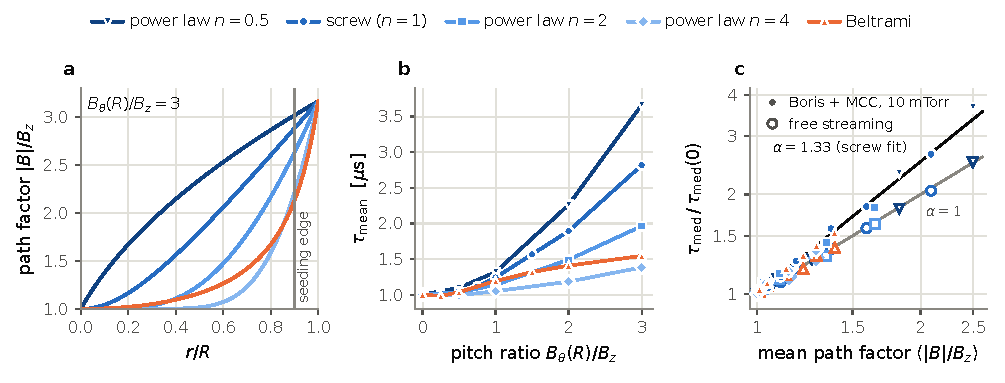
\includegraphics[width=\textwidth]{figures/pitch-transport-law.pdf}
\caption{Test-particle transport at the baseline (argon, 10~mTorr, $|B(R)| = 100$~G, electrons seeded at 3~eV). (a)~Local path factor $|B|/B_z$ of the five twist profiles at $\Theta = 3$. All reach $\sqrt{10}$ at the wall and differ in where the twist sits; particles are seeded inside $r = 0.9R$. (b)~Mean confinement time against pitch ratio, with one-standard-error bars. All profiles are the same uniform field at $\Theta = 0$, and the Beltrami curve starts from that common point. (c)~Median confinement time, normalized to its value at $\Theta = 0$, against the seeding-averaged path factor of Eq.~\eqref{eq:meanF}. Filled markers: Boris pusher with Monte Carlo collisions. Open markers: free-streaming geometric model. Lines: the power law fitted to the screw profile alone ($\alpha = 1.33$) and $\alpha = 1$.}
\label{fig:law}
\end{figure}

\begin{table}[htbp]
\centering
\caption{Mean electron confinement time $\tau_{\mathrm{mean}}$ (\us) at the baseline ($N = 4000$ per point; standard errors 0.02--0.06~\us). All profiles are the same uniform field at $\Theta = 0$. The lower rows give the seeding-averaged path factor at $\Theta = 3$ and the exponent of Eq.~\eqref{eq:law} fitted to medians, with collisions and in the free-streaming model.}
\label{tab:scan}
\begin{tabular}{lccccc}
\toprule
 & \multicolumn{4}{c}{power law, $B_\theta \propto r^n$} & \\
\cmidrule(lr){2-5}
$\Theta$ & $n = 0.5$ & $n = 1$ (screw) & $n = 2$ & $n = 4$ & Beltrami \\
\midrule
0   & 1.00 & 1.00 & 1.00 & 1.00 & 1.00 \\
0.5 & 1.10 & 1.02 & 1.03 & 0.99 & 1.04 \\
1   & 1.32 & 1.24 & 1.14 & 1.05 & 1.19 \\
2   & 2.26 & 1.89 & 1.49 & 1.18 & 1.41 \\
3   & 3.66 & 2.82 & 1.96 & 1.38 & 1.54 \\
\midrule
$\langle F\rangle$ at $\Theta = 3$ & 2.50 & 2.09 & 1.65 & 1.29 & 1.39 \\
$\alpha$, Boris + MCC & $1.41 \pm 0.04$ & $1.33 \pm 0.03$ & $1.16 \pm 0.05$ & $1.15 \pm 0.07$ & $1.25 \pm 0.02$ \\
$\alpha$, free streaming & $0.99 \pm 0.01$ & $0.97 \pm 0.02$ & $0.95 \pm 0.03$ & $0.95 \pm 0.05$ & $0.97 \pm 0.05$ \\
\bottomrule
\end{tabular}
\end{table}

\subsection{Mechanism}
\label{sec:mechanism}

To locate the mechanism, physics is added one ingredient at a time from identical seeding (Table~\ref{tab:layers}). The bottom layer is a free-streaming geometric model that integrates nothing: each electron moves along its field line at constant $v_\parallel$, and its loss time is its axial distance to the end plate divided by $|v_\parallel|\,B_z/|B|$, censored exactly as in the particle runs. The second layer is the Boris pusher with collisions switched off, which adds gyration and the grad-$B$ and curvature drifts. The third adds collisions.

\begin{table}[htbp]
\centering
\caption{Mechanism decomposition for the screw field at the baseline: confinement at $\Theta = 0$ and 3 and the resulting pitch gain. Means and medians are both shown because the layers weight the slow-$v_\parallel$ tail differently (the free-streaming model uses $N = 20000$); medians are the robust comparison.}
\label{tab:layers}
\begin{tabular}{lcccccc}
\toprule
 & \multicolumn{3}{c}{$\tau_{\mathrm{mean}}$ (\us)} & \multicolumn{3}{c}{$\tau_{\mathrm{med}}$ (\us)} \\
\cmidrule(lr){2-4}\cmidrule(lr){5-7}
layer & $\Theta = 0$ & $\Theta = 3$ & gain & $\Theta = 0$ & $\Theta = 3$ & gain \\
\midrule
free streaming (geometry only) & 1.35 & 2.41 & 1.78 & 0.384 & 0.788 & 2.05 \\
Boris, no collisions (+ gyration, drifts) & 1.21 & 2.43 & 2.01 & 0.391 & 0.797 & 2.04 \\
Boris + MCC (+ collisions) & 1.00 & 2.82 & 2.81 & 0.662 & 1.753 & 2.65 \\
\bottomrule
\end{tabular}
\end{table}

Three conclusions follow. \emph{Drifts are negligible at 100~G}: collisionless Boris medians agree with free streaming to within 3.2\% at every pitch ratio for both the screw and Beltrami fields, and the collisionless radial loss is exactly zero. \emph{Geometry sets the shape}: free streaming reproduces the flat-then-linear dependence on $\Theta$ and the ordering of profiles; for example, it gives 1.78~\us{} for the Beltrami field at $\Theta = 3$ against 2.41~\us{} for the screw field. \emph{Collisions amplify the effect}: at 3~eV the electron mean free path, $(n_n\sigma)^{-1} \approx 16$~cm, is a fraction of the 40~cm chamber length, so parallel transport is marginally diffusive and residence time grows faster than linearly with path length. The median gain rises from 2.05 to 2.65.

\subsection{A geometric transport law}
\label{sec:law}

Combining profiles and collisionalities, the median confinement time follows
\begin{equation}
\tau_{\mathrm{med}} \approx \tau_0\,\langle F\rangle^{\alpha}, \qquad \alpha = \alpha(L/\lambda_{\mathrm{mfp}}),
\label{eq:law}
\end{equation}
in which the whole field geometry enters through the single scalar of Eq.~\eqref{eq:meanF} (Fig.~\ref{fig:law}c). Without collisions $\alpha = 1$, as free streaming requires: median fits give 0.95--0.99 in the free-streaming model for all five profiles, and 0.96 and 0.94 for the collisionless Boris runs of the screw and Beltrami fields. With collisions $\alpha$ grows toward the diffusive limit of 2 as parallel collisionality increases (Table~\ref{tab:params}). It does so both with pressure---1.19, 1.33, and 1.39 at 3, 10, and 30~mTorr---and with electron energy through $\sigma(E)$: at 1~eV, near the Ramsauer--Townsend minimum, the least collisional case gives 1.17, while 10~eV gives 1.45. At fixed pressure the five profiles give 1.15--1.41, and this spread sets the present precision of a single-exponent law.

The law's predictive content is tested out of sample (Table~\ref{tab:predict}). The exponent and prefactor fitted to the eight screw-field medians predict the medians of the other profiles, none of which enter the fit. For the Beltrami field the prediction is within 2\% at all five pitch ratios from 0.5 to 3; for the power-law profiles it is within $-8\%$ to $+6\%$. The two tests probe different things. The Beltrami field has a different functional form but spans only $\langle F\rangle \le 1.39$, where exponents between 1.25 and 1.33 are hard to distinguish. The $n = 0.5$ profile reaches $\langle F\rangle = 2.50$, beyond the range of the screw fit, and shows the largest deviation.

\begin{table}[htbp]
\centering
\caption{Out-of-sample test of Eq.~\eqref{eq:law} at $\Theta = 3$. The exponent ($\alpha = 1.33$) and prefactor are fitted to the eight screw-field medians alone and applied to the other profiles. Across all pitch ratios $\Theta \ge 0.5$ the Beltrami errors are within $\pm2\%$ and the power-law errors within $-8\%$ to $+6\%$.}
\label{tab:predict}
\begin{tabular}{lcccc}
\toprule
profile & $\langle F\rangle$ & predicted $\tau_{\mathrm{med}}$ (\us) & measured $\tau_{\mathrm{med}}$ (\us) & error \\
\midrule
screw (in the fit) & 2.09 & 1.77 & 1.75 & $+1\%$ \\
power law, $n = 0.5$ & 2.50 & 2.24 & 2.43 & $-8\%$ \\
power law, $n = 2$ & 1.65 & 1.29 & 1.21 & $+6\%$ \\
power law, $n = 4$ & 1.29 & 0.93 & 0.89 & $+4\%$ \\
Beltrami & 1.39 & 1.03 & 1.01 & $+1\%$ \\
\bottomrule
\end{tabular}
\end{table}

\subsection{Loss channels and parameter dependence}
\label{sec:topology}

Table~\ref{tab:params} separates the loss channels using the channel rates $\Gamma_{\mathrm{ch}} = f_{\mathrm{ch}}/\tau_{\mathrm{mean}}$, where $f_{\mathrm{ch}}$ is the fraction of electrons lost through each channel. Under every condition the whole confinement gain is suppression of end loss, with $\Gamma_{\mathrm{end}}$ falling by a factor of 2.3--3.4. The radial channel is parasitic. It rises with pitch and with collisionality and falls steeply with field strength, as expected for collisional cross-field steps of order the gyroradius accumulated over a longer dwell time. At the baseline it is 40 times smaller than the end channel at $\Theta = 3$, but it reaches 8--11\% of it at 50~G, 30~mTorr, or 10~eV, and it must eventually limit the gain. Field strength sets no axial timescale---$\tau(0) = 0.96$--1.00~\us{} from 50 to 200~G---as the geometric mechanism requires. Pitch leverage grows with collisionality, from $2.33\times$ at 3~mTorr to $2.95\times$ at 30~mTorr and from $2.33\times$ at 1~eV to $3.12\times$ at 10~eV, so the effect on test particles is strongest in the collisional regime where processing plasmas operate.

\begin{table}[htbp]
\centering
\small
\setlength{\tabcolsep}{4.5pt}
\caption{Parameter dependence and loss channels for the screw field, one factor varied at a time from the baseline (10~mTorr, 3~eV, 100~G; $N = 4000$). Channel rates $\Gamma_{\mathrm{ch}} = f_{\mathrm{ch}}/\tau_{\mathrm{mean}}$ are given at $\Theta = 0$ and 3.}
\label{tab:params}
\begin{tabular}{lccccccc}
\toprule
condition & $\tau(0)$ (\us) & $\tau(3)$ (\us) & gain & $\alpha$ (median) & $\Gamma_{\mathrm{end}}$ (\us$^{-1}$) & $\Gamma_{\mathrm{rad}}$ ($10^{-3}$\,\us$^{-1}$) & $\Gamma_{\mathrm{rad}}/\Gamma_{\mathrm{end}}$ at 3 \\
\midrule
baseline & 1.00 & 2.82 & 2.81 & $1.33 \pm 0.03$ & $0.99 \to 0.35$ & $4.0 \to 8.8$ & 2.5\% \\
3~mTorr  & 0.80 & 1.85 & 2.33 & $1.19 \pm 0.03$ & $1.26 \to 0.54$ & $0.0 \to 1.2$ & 0.2\% \\
30~mTorr & 1.68 & 4.96 & 2.95 & $1.39 \pm 0.05$ & $0.58 \to 0.18$ & $13.8 \to 20.0$ & 11\% \\
1~eV     & 1.36 & 3.17 & 2.33 & $1.17 \pm 0.01$ & $0.73 \to 0.32$ & $0.0 \to 0.1$ & $<0.1\%$ \\
10~eV    & 0.93 & 2.91 & 3.12 & $1.45 \pm 0.02$ & $1.05 \to 0.31$ & $17.7 \to 32.2$ & 10\% \\
50~G     & 0.96 & 2.59 & 2.69 & $1.28 \pm 0.03$ & $1.02 \to 0.36$ & $16.1 \to 28.9$ & 8.1\% \\
200~G    & 0.98 & 3.01 & 3.06 & $1.37 \pm 0.04$ & $1.02 \to 0.33$ & $0.0 \to 1.7$ & 0.5\% \\
\bottomrule
\end{tabular}
\end{table}

\paragraph{An end-plate asymmetry.} At high pitch, collisional runs lose more electrons through the $z = 0$ end plate than through $z = L$. At $\Theta = 3$ the difference between the two end-plate loss fractions reaches 0.12--0.13 (8--9 standard deviations) at 30~mTorr and 10~eV, and 0.11 (7 standard deviations) for the $n = 0.5$ profile. At $\Theta = 0$ it is at most 0.03 (2 standard deviations), and in the collisionless run at $\Theta = 3$ it is $-0.015$. These observations are consistent with symmetry. At zero pitch the configuration is invariant under the reflection $z \to -z$. Without collisions, a free-streaming electron's exit direction is set by the sign of $v_\parallel$, which is symmetric in the seeded Maxwellian. A twisted field has a handedness, and with collisions neither argument applies. Runs that share a seed and scan index start from the same ensemble, so these values are not independent; the independent seed-2 baseline gives $+0.06$ (4 standard deviations). We have not identified the mechanism, and the asymmetry does not affect the totals above.

\section{Self-consistent electrostatic fields}
\label{sec:selfconsistent}

Section~\ref{sec:testparticle} treats electrons as independent particles in a vacuum field. In a plasma their escape charges the column, and the resulting potential acts back on the electrons that remain. This section adds that feedback in the three stages of Section~\ref{sec:poisson}, all for the screw field.

\subsection{Frozen ions}
\label{sec:frozen}

With the field switched off, the self-consistent runner reproduces the test-particle result: $\tau_{\mathrm{mean}} = 1.02$, 1.19, and 2.76~\us{} at $\Theta = 0$, 1, and 3, a gain of $2.71\times$. With the field on, escape of the fast tail charges the column to an 11.5~V ($3.8\,T_e$) potential well that returns slower electrons. Confinement lengthens by a factor of at least 6.8 at $\Theta = 0$ and 2.9 at $\Theta = 3$---22--24\% of electrons remain at 20~\us, against under 0.5\% without the field---and the pitch gain collapses to $1.17\times$ in censored means, with survival at 20~\us{} rising only from 22.3 to 24.2\% between $\Theta = 0$ and 3.

The well reaches 85\% of the full-depletion potential of 13.6~V, which raises the question of whether that cap sets the result. Doubling $n_0$ raises the cap to 27.1~V; the well deepens to 18.3~V ($6.1\,T_e$, 67\% of the new cap), and the gain is again $1.17\times$ (10~\us{} horizon). Within this factor of two, the compression is not an artifact of the cap.

Table~\ref{tab:frozen} resolves the structure of the well over six pitch ratios. The well does not respond to geometry: its peak scatters by $\pm7\%$ without trend, and its radial half-width (6.1--6.8~cm) and axial width (29--30~cm) are fixed. What pitch does change is the late-time leak of the trapped population. The e-folding time $\tau_{\mathrm{leak}}$ falls monotonically from 34.8 to 17.6~\us{} as the radial share of losses grows from 0.3 to 3.8\%, so in this regime pitch trades a modest early gain for a faster late drain. Single density snapshots from these decaying runs are too noisy to resolve structural change: the core inventory share defined in Section~\ref{sec:sustained} differs by up to 0.07 between the two halves of its averaging band.

\begin{table}[htbp]
\centering
\small
\caption{Frozen-ion electrostatic feedback, screw field at the baseline ($N = 2000$, 10~\us{} horizon; potential from the final snapshot). $\phi_{\max}$: peak potential. $\phi_{\mathrm{plat}}$: on-axis potential averaged over the central half of $z$. $r_{1/2}$: radius at which the midplane potential falls to $\phi_{\max}/2$. $z$ FWHM: on-axis full width at half maximum. Survival: electrons remaining at 10~\us. $\tau_{\mathrm{leak}}$: e-folding time of the surviving population over the second half of the run. Radial: share of lost electrons that reached the radial wall.}
\label{tab:frozen}
\begin{tabular}{cccccccc}
\toprule
$\Theta$ & $\phi_{\max}$ (V) & $\phi_{\mathrm{plat}}$ (V) & $r_{1/2}$ (cm) & $z$ FWHM (cm) & survival & $\tau_{\mathrm{leak}}$ (\us) & radial \\
\midrule
0   & 9.31  & 8.10 & 6.6 & 30.0 & 32.0\% & 34.8 & 0.3\% \\
0.5 & 9.53  & 8.23 & 6.4 & 30.0 & 31.8\% & 33.9 & 0.6\% \\
1   & 9.13  & 8.05 & 6.6 & 30.0 & 33.0\% & 28.6 & 1.0\% \\
1.5 & 9.34  & 8.55 & 6.8 & 30.0 & 30.3\% & 22.3 & 1.3\% \\
2   & 8.73  & 7.91 & 6.8 & 30.0 & 33.6\% & 20.6 & 2.9\% \\
3   & 10.01 & 8.63 & 6.1 & 29.2 & 34.9\% & 17.6 & 3.8\% \\
\bottomrule
\end{tabular}
\end{table}

\subsection{Mobile ions and the exit-speed Hall parameter}
\label{sec:mobile}

Frozen ions cannot respond to pitch. At 100~G and 10~mTorr real argon ions are unmagnetized ($H_i \approx 0.19$ \cite{auerbach2026}), and in a steady discharge the bulk loss rate follows the slower ion channel, which is blind to pitch below ion magnetization. The frozen-ion result therefore suggested a regime-gated hypothesis: pitch control of bulk confinement should switch on once the ions are magnetized. The mobile-ion scans test it.

With mobile ions the well relaxes to about 6~V at 100~G, and ion escape sets the slow decay. At 10~mTorr (Table~\ref{tab:mobile}) the thermal Hall parameter spans 0.3--4.8, yet the pitch gain stays between 1.12 and 1.32 with no threshold, while ion survival at 25~\us{} rises with field from 23 to 69\% independently of pitch. The thermal parameter overstates how magnetized the escaping ions are, because they leave at about $c_s$ (Section~\ref{sec:hall}); in this scan $H_i^*$ never exceeded 0.70. The 3~mTorr scan carries $H_i^*$ through unity to 2.35, and there the gain declines monotonically from 1.15 to 0.97 (Fig.~\ref{fig:gain}). The strong form of the hypothesis---that the bulk confinement gain re-emerges above ion magnetization---is not supported. A weak form is: at $H_i^* = 2.35$ the ion channel itself becomes pitch-sensitive, with ion survival rising from 71.5 to 78.1\% between $\Theta = 0$ and 3 while electron survival falls from 13.3 to 9.3\%.

These decaying ensembles locate trends, not equilibrium values. They are far from flux balance ($\Gamma_i/\Gamma_e = 1.35$--3.35), electron survival at 25~\us{} is only 0.3--13\%, and each point is a single seed with $N = 1000$ per species. The sustained runs remove the first two limitations.

\begin{table}[htbp]
\centering
\small
\caption{Decaying ensembles with mobile 1-amu ions (screw field, $N = 1000$ per species, 25~\us{} horizon). The gain is the ratio of censored mean electron confinement times at $\Theta = 3$ and 0. Survival fractions are at 25~\us. $\Gamma_i/\Gamma_e$ is the ion-to-electron wall-flux ratio over the second half of the run at $\Theta = 0$; it would be 1 in a balanced steady state.}
\label{tab:mobile}
\begin{tabular}{cccccccc}
\toprule
$p$ & $B$ & & & & \multicolumn{2}{c}{survival at 25~\us, $\Theta = 0 \to 3$} & \\
\cmidrule(lr){6-7}
(mTorr) & (G) & $H_i$ & $H_i^*$ & gain & electrons & ions & $\Gamma_i/\Gamma_e$ \\
\midrule
10 & 25  & 0.30  & 0.04 & 1.15 & $4.5 \to 3.1\%$   & $23.3 \to 24.0\%$ & 2.76 \\
10 & 50  & 0.59  & 0.09 & 1.24 & $1.5 \to 0.7\%$   & $22.2 \to 21.8\%$ & 3.35 \\
10 & 100 & 1.19  & 0.18 & 1.32 & $1.5 \to 1.9\%$   & $25.0 \to 26.1\%$ & 2.88 \\
10 & 200 & 2.38  & 0.35 & 1.24 & $2.4 \to 3.3\%$   & $38.6 \to 36.5\%$ & 2.25 \\
10 & 400 & 4.76  & 0.70 & 1.12 & $10.7 \to 8.8\%$  & $68.8 \to 66.8\%$ & 1.73 \\
\midrule
3  & 50  & 1.98  & 0.29 & 1.15 & $1.2 \to 0.3\%$   & $12.9 \to 11.3\%$ & 3.02 \\
3  & 100 & 3.96  & 0.59 & 1.12 & $1.5 \to 1.1\%$   & $21.3 \to 19.9\%$ & 2.66 \\
3  & 200 & 7.93  & 1.17 & 1.05 & $4.0 \to 2.3\%$   & $43.3 \to 42.8\%$ & 2.32 \\
3  & 400 & 15.86 & 2.35 & 0.97 & $13.3 \to 9.3\%$  & $71.5 \to 78.1\%$ & 1.35 \\
\bottomrule
\end{tabular}
\end{table}

\begin{figure}[htbp]
\centering
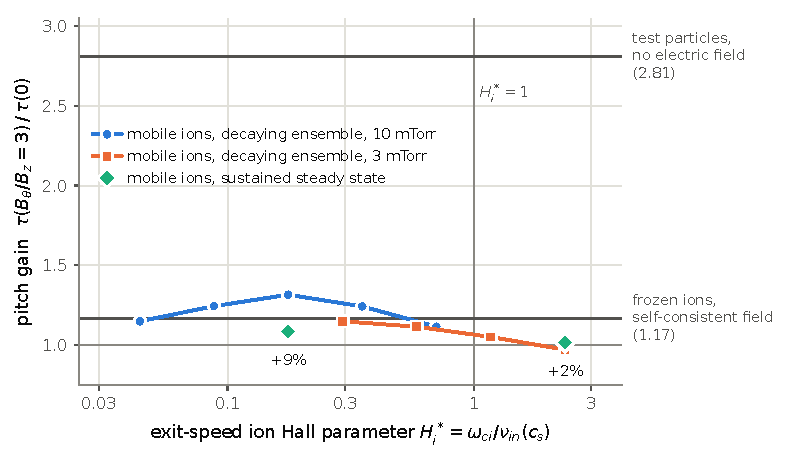
\includegraphics[width=0.82\textwidth]{figures/pitch-gain-hierarchy.pdf}
\caption{Pitch gain $\tau(\Theta = 3)/\tau(0)$ as the model gains self-consistency. Horizontal lines: test particles with no electric field (screw field, 10~mTorr) and electrons in a self-consistent field over frozen ions (20~\us{} horizon). Circles and squares: decaying ensembles with mobile 1-amu ions, scanned in $B$ at 10 and 3~mTorr and plotted against the exit-speed ion Hall parameter; gains are ratios of censored mean electron confinement times. Diamonds: source-sustained steady state, where $\tau$ is the uncensored $\tau_{\mathrm{eff}} = \langle N_e\rangle/S$, at 100~G, 10~mTorr and 400~G, 3~mTorr. Each point is a single run; the $-2\%$ change at $\Theta = 1$ in the sustained 100~G run indicates variation of a few percent.}
\label{fig:gain}
\end{figure}

\subsection{Source-sustained steady state}
\label{sec:sustained}

In source-sustained steady state the plasma fills until its losses balance the source. The wall-flux ratio is then 0.89--1.01 in every run, and confinement is measured without censoring. Table~\ref{tab:sustained} and Figs.~\ref{fig:gain} and~\ref{fig:structure} summarize the two conditions, 100~G at 10~mTorr ($H_i^* = 0.18$) and 400~G at 3~mTorr ($H_i^* = 2.35$). Three results close the self-consistent study.

\emph{Bulk confinement is nearly independent of pitch.} Between $\Theta = 0$ and 3, $\tau_{\mathrm{eff}}$ changes by $+9\%$ below ion magnetization and by $+2\%$ above it, against $2.81\times$ for test particles. At 100~G the intermediate ratio gives $-2\%$, an indication of run-to-run variation of a few percent.

\emph{Pitch changes how the plasma is confined, not how well.} At both conditions the plateau potential falls with pitch---by 12\% at 100~G and 11\% at 400~G---while the radial and axial widths of the well are unchanged to within 0.4 and 1.7~cm. Longer magnetic paths substitute for part of the electrostatic barrier at nearly fixed confinement (Section~\ref{sec:discussion}). At 100~G pitch also shifts electron loss toward the radial wall (from 0.3 to 2.4\% of losses); at 400~G all electron losses remain at the end plates.

\emph{The equilibrium density redistributes, and more strongly above ion magnetization.} We measure structure by the core inventory share $f_{\mathrm{core}}$, the fraction of electrons at $r < 0.4R$ in the density averaged over the central half of the chamber length. As an integral it is far less sensitive to per-cell sampling noise than a peak radius, and its values over the two halves of the averaging band agree to within 0.008 in every sustained run. At $\Theta = 3$, $f_{\mathrm{core}}$ falls by 20\% at $H_i^* = 0.18$ and by 34\% at $H_i^* = 2.35$, while the intermediate ratio at 100~G leaves it unchanged. The response is visible directly in Fig.~\ref{fig:structure}b, where high pitch roughly halves the core density and leaves the edge unchanged. The two conditions differ in both $B$ and $p$, so a fixed-pressure field scan is needed to attribute the stronger response to ion magnetization alone.

\begin{table}[htbp]
\centering
\small
\setlength{\tabcolsep}{4.5pt}
\caption{Source-sustained steady state (mobile 1-amu ions, screw field; averages over the second half of each run). $\tau_{\mathrm{eff}} = \langle N_e\rangle/S$. $\phi_{\mathrm{plat}}$: on-axis potential averaged over the central half of $z$. $\Gamma_i/\Gamma_e$: ion-to-electron wall-flux ratio. $N_i/N_e$: steady inventory ratio. $f_{\mathrm{core}}$: share of the electron inventory at $r < 0.4R$ over the central half of $z$. Changes are relative to $\Theta = 0$ at the same condition; single seed per point.}
\label{tab:sustained}
\begin{tabular}{llcccccccc}
\toprule
condition & $\Theta$ & $\tau_{\mathrm{eff}}$ (\us) & change & $\phi_{\mathrm{plat}}$ (V) & change & $\Gamma_i/\Gamma_e$ & $N_i/N_e$ & $f_{\mathrm{core}}$ & change \\
\midrule
100~G, 10~mTorr    & 0 & 8.54  & ---      & 4.28 & ---       & 1.01 & 1.79 & 0.175 & ---       \\
($H_i^* = 0.18$)   & 1 & 8.35  & $-2\%$   & 4.22 & $-1\%$    & 1.00 & 1.80 & 0.173 & $-1\%$    \\
                   & 3 & 9.28  & $+9\%$   & 3.76 & $-12\%$   & 1.00 & 1.67 & 0.140 & $-20\%$   \\
\midrule
400~G, 3~mTorr     & 0 & 15.49 & ---      & 8.04 & ---       & 0.93 & 1.73 & 0.195 & ---       \\
($H_i^* = 2.35$)   & 3 & 15.75 & $+2\%$   & 7.17 & $-11\%$   & 0.89 & 1.79 & 0.129 & $-34\%$   \\
\bottomrule
\end{tabular}
\end{table}

\begin{figure}[htbp]
\centering
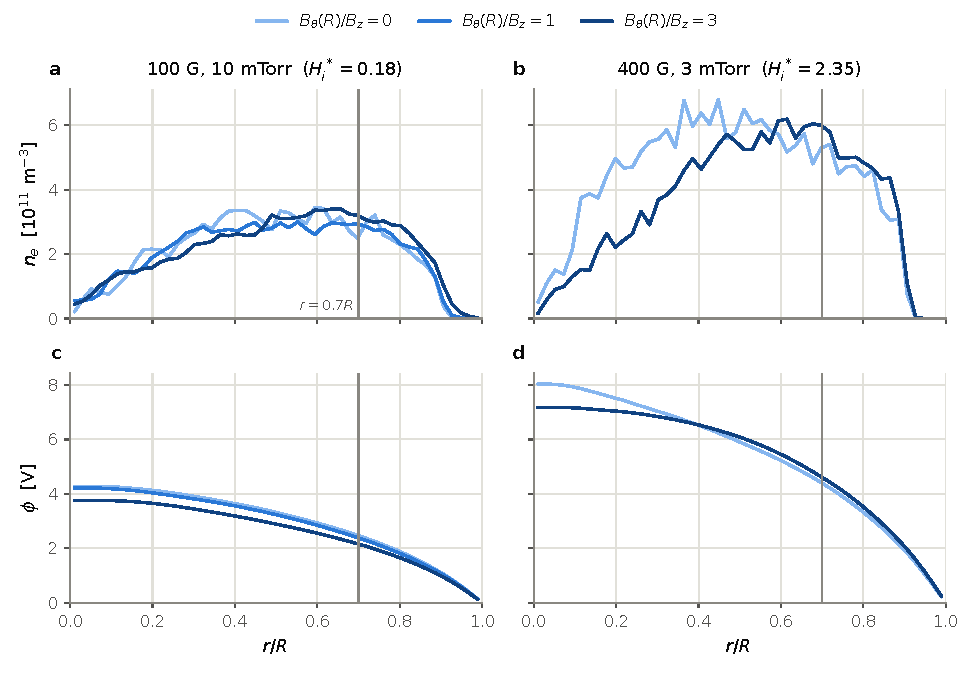
\includegraphics[width=\textwidth]{figures/pitch-equilibrium-structure.pdf}
\caption{Equilibrium structure of the source-sustained runs, averaged over the second half of each run and over the central half of the chamber length. (a,~b)~Electron density; (c,~d)~electrostatic potential. Left: 100~G, 10~mTorr ($H_i^* = 0.18$). Right: 400~G, 3~mTorr ($H_i^* = 2.35$). The vertical line marks $r = 0.7R$. Densities near the axis come from small cell volumes and carry the largest sampling noise; the integral measure $f_{\mathrm{core}}$ of Table~\ref{tab:sustained} is insensitive to it.}
\label{fig:structure}
\end{figure}

\section{Discussion}
\label{sec:discussion}

\subsection{Why the confinement gain does not survive}

Connection length is a property of electron orbits, whereas bulk confinement is a property of the coupled electron--ion system. Once space charge is included, faster electron loss charges the column positive until the potential throttles electron escape to what the ions allow, and in steady state the two wall fluxes are equal. If the ion loss rate does not depend on pitch, as for unmagnetized ions, then neither can the bulk particle confinement time. Lengthening the electron paths instead lowers the potential needed to hold the electrons. This is what the sustained runs show: the plateau potential drops by 11--12\% at $\Theta = 3$ while $\tau_{\mathrm{eff}}$ changes by $+2$ to $+9\%$, so magnetic path length substitutes for part of the electrostatic barrier. We do not attempt a quantitative barrier balance, because at $R/\lambda_D \approx 3$ the potential is set by the net space charge of the whole column rather than by a Boltzmann relation at a sheath.

Crossing ion magnetization was expected to break this argument by making the ion channel pitch-sensitive. It did make the ion channel pitch-sensitive, but in the coupled system the change appeared as a shallower well and a redistributed density, not as longer bulk confinement.

The boundary conditions matter. Grounded conducting walls and end plates allow electrons and ions to leave through different surfaces, with the difference in currents closing through the wall---the short-circuit effect identified by Simon \cite{simon1955}, which is central to transport in finite-length magnetized columns \cite{curreli2014}. Insulating end plates force the electron and ion fluxes to balance along each field line and remove that freedom; they are the most direct test of how general the present verdict is.

\subsection{Implications for pitch-controlled sources}

Prediction~4 of Ref.~\cite{auerbach2026} states that a pitch scan at constant $|B|$ and power should change the coupled power and the density profile. The present model has no RF coupling and says nothing about the first part. It supports the second, but through structure rather than confinement. If the transport results carry over to quasineutral discharges (Section~\ref{sec:limitations}), an experiment at fixed $|B|$, pressure, and RF power should find the following.
\begin{enumerate}
  \item Bulk density changes with pitch by about 10\% or less through transport alone.
  \item The plasma potential falls with pitch, by of order 10\% at $\Theta = 3$, measurable with emissive or floating probes.
  \item The share of density in the core falls with pitch, by roughly 20\% below ion magnetization and more above it, measurable with radial Langmuir probe arrays \cite{hutchinson}.
  \item The stronger structural response requires $H_i^* \gtrsim 1$, which for argon means about 3.6~kG at 10~mTorr but 1.1~kG at 3~mTorr, so fill pressure is part of the design space.
\end{enumerate}
A bulk-density response much larger than 10\% would therefore point to a pathway absent from this model. The obvious candidate is pitch-dependent power deposition, since helicon wave propagation and antenna coupling depend on the field geometry \cite{chenarnush1997,chen2015}.

\section{Limitations}
\label{sec:limitations}

The conclusions above hold within a reduced model, and its main simplifications are listed here in rough order of importance.
\begin{enumerate}
  \item \textbf{Space-charge-limited regime.} The self-consistent runs sit at volume-averaged electron densities of $1.6$--$3.1\times10^{11}$~m$^{-3}$, with $R/\lambda_D \approx 3$--4 and $N_i/N_e \approx 1.7$--1.8. Processing and helicon plasmas are quasineutral at $10^{16}$--$10^{18}$~m$^{-3}$, with thin sheaths. The flux-balance argument of Section~\ref{sec:discussion} does not depend on density, but the well depth, the size of the potential--path-length substitution, and the structural response may. An implicit or quasineutral formulation is needed to test this.
  \item \textbf{No heating or wave coupling.} Electrons only cool, ionization produces no pairs, and the steady state is sustained by an imposed source rather than by the discharge itself. Any pitch dependence of RF power deposition is absent by construction.
  \item \textbf{Reduced ion mass.} The mobile-ion studies use a 1-amu model gas. Results are indexed by $H_i^*$, but ion mass also enters the sheath potential and the ion transit time, so the translation to argon is not exact.
  \item \textbf{Collision data.} The cross sections are representative tables, there is no excitation channel, ion cross sections are energy-independent, and there are no Coulomb collisions or neutral depletion.
  \item \textbf{Boundaries.} All surfaces are grounded conductors with no secondary emission, no bias, and no floating or insulating end plates.
  \item \textbf{Idealized fields.} The helical profiles have $B_r = 0$ and no end effects, ripple, or coil-set structure, and the model is electrostatic, with no self-generated magnetic perturbation or inductive field.
  \item \textbf{Statistics and design.} Each self-consistent point is a single seed; decaying ensembles use $N = 1000$--2000; the sustained comparison varies $B$ and $p$ together; and no error bars are available for $\tau_{\mathrm{eff}}$ beyond the few-percent variation indicated by the intermediate ratio.
\end{enumerate}

\section{Conclusions}
\label{sec:conclusions}

In test-particle transport, field-line pitch is a strong and lawful control on electron confinement. Confinement grows as a power of the seeding-averaged path factor $\langle|B|/B_z\rangle$, with an exponent that rises from 1 toward 2 with parallel collisionality; it depends as much on where the twist sits as on how much there is; and it acts entirely by suppressing end loss. When the plasma's own electrostatic field is included, the bulk confinement gain does not survive. It collapses from $2.8\times$ to $1.17\times$ with frozen ions, and to $+9\%$ and $+2\%$ in sustained steady state on both sides of an ion-magnetization boundary that is located by the exit-speed Hall parameter $H_i^*$ rather than the thermal $H_i$. Pitch does act on the equilibrium: it lowers the confining potential at nearly fixed confinement, moves losses between channels and species, and moves electron inventory out of the core, most strongly above ion magnetization.

Within this model, then, pitch is a structural control parameter rather than a confinement parameter. The verdict rests on a space-charge-limited, electrostatic, source-sustained model without RF heating. The next steps are chosen to test it where it is weakest: a fixed-pressure field scan of the equilibrium structure across $H_i^* = 1$, insulating end plates, a quasineutral or implicit formulation that reaches realistic densities, and a coupling model for pitch-dependent RF power deposition.

% \section*{Acknowledgments}
% TODO(author): acknowledgments, and any AI-assistance disclosure your target venue requires.

\section*{Code and data availability}

\begin{sloppypar}
The simulator, the archived runs behind every table and figure (\texttt{paper/data/}), and the script that regenerates the figures and prints every derived number quoted here (\texttt{paper/figures/pitch\_figures.py}) are openly available at \url{https://github.com/ZachBach/ElectromagneticHelixReactor}. The physics self-test runs with \texttt{npm run sim:selftest}. Table~\ref{tab:manifest} lists the runs.
\end{sloppypar}

\appendix

\section{Run manifest}
\label{sec:manifest}

\begin{table}[htbp]
\centering
\small
\caption{Runs used in this paper. All use argon, $R = 0.1$~m, $L = 0.4$~m, 3~eV electron seeding, and seed 1 unless noted. The CSV outputs are archived in \texttt{paper/data/}; each file's header records its full parameter set.}
\label{tab:manifest}
\begin{tabular}{>{\raggedright}p{2.6cm}>{\raggedright}p{4.3cm}>{\raggedright}p{5.6cm}>{\raggedright\arraybackslash}p{2.2cm}}
\toprule
study & runner & parameters & used in \\
\midrule
pitch scans & \texttt{run-pitch-scan.js} & five profiles; 100~G, 10~mTorr; $N = 4000$, $T_{\max} = 50$~\us & Tables~\ref{tab:scan}, \ref{tab:predict}; Fig.~\ref{fig:law} \\
collisionless & \texttt{run-pitch-scan.js -{}-nocoll} & screw and Beltrami & Table~\ref{tab:layers} \\
free streaming & \texttt{mechanism.js} & five profiles; $N = 20000$ & Table~\ref{tab:layers}; Fig.~\ref{fig:law}c \\
parameter scans & \texttt{run-pitch-scan.js} & $p = 3, 30$~mTorr; $T_e = 1, 10$~eV; $|B(R)| = 50, 200$~G; $\Theta = 0, 0.5, 1, 2, 3$ & Table~\ref{tab:params} \\
convergence & \texttt{run-pitch-scan.js} & $\Delta t/2$ at $\Theta = 0, 1, 3$; seed 2 & Section~\ref{sec:verification} \\
frozen ions & \texttt{run-ambipolar.js} & field off and on, $N = 2000$, 20~\us; $n_0 = 6\times10^{11}$~m$^{-3}$, 10~\us; six pitch ratios, 10~\us & Table~\ref{tab:frozen}; Fig.~\ref{fig:gain} \\
mobile ions & \texttt{run-ambipolar.js -{}-ions=mobile -{}-mion=1} & 25--400~G at 10~mTorr and 50--400~G at 3~mTorr; $\Theta = 0, 3$; $N = 1000$, 25~\us & Table~\ref{tab:mobile}; Fig.~\ref{fig:gain} \\
sustained & \texttt{run-sustained.js -{}-mion=1} & 100~G, 10~mTorr, $\Theta = 0, 1, 3$, 50~\us; 400~G, 3~mTorr, $\Theta = 0, 3$, 40~\us; 200 pairs/\us & Table~\ref{tab:sustained}; Figs.~\ref{fig:gain}, \ref{fig:structure} \\
\bottomrule
\end{tabular}
\end{table}

\begin{thebibliography}{99}
\bibitem{lieberman} M.~A. Lieberman and A.~J. Lichtenberg, \textit{Principles of Plasma Discharges and Materials Processing}, 2nd ed., Wiley, 2005.
\bibitem{chabert} P.~Chabert and N.~Braithwaite, \textit{Physics of Radio-Frequency Plasmas}, Cambridge University Press, 2011.
\bibitem{chen2015} F.~F. Chen, ``Helicon discharges and sources: a review,'' \textit{Plasma Sources Sci. Technol.} \textbf{24}, 014001 (2015).
\bibitem{curreli2014} D.~Curreli and F.~F. Chen, ``Cross-field diffusion in low-temperature plasma discharges of finite length,'' \textit{Plasma Sources Sci. Technol.} \textbf{23}, 064001 (2014).
\bibitem{stangeby} P.~C. Stangeby, \textit{The Plasma Boundary of Magnetic Fusion Devices}, Institute of Physics Publishing, 2000.
\bibitem{auerbach2026} Z.~Auerbach, ``Electromagnetic Helix Reactor (EHR): A Multi-Physics Plasma Control Architecture for Advanced Plasma Processing,'' unpublished preprint (2026), \url{https://github.com/ZachBach/ElectromagneticHelixReactor}.
\bibitem{simon1955} A.~Simon, ``Ambipolar diffusion in a magnetic field,'' \textit{Phys. Rev.} \textbf{98}, 317 (1955).
\bibitem{taylor1974} J.~B. Taylor, ``Relaxation of toroidal plasma and generation of reverse magnetic fields,'' \textit{Phys. Rev. Lett.} \textbf{33}, 1139 (1974).
\bibitem{freidberg} J.~P. Freidberg, \textit{Ideal MHD}, Cambridge University Press, 2014.
\bibitem{boris1970} J.~P. Boris, ``Relativistic plasma simulation---optimization of a hybrid code,'' in \textit{Proceedings of the Fourth Conference on Numerical Simulation of Plasmas}, Naval Research Laboratory, Washington, DC, 1970, pp.~3--67.
\bibitem{qin2013} H.~Qin, S.~Zhang, J.~Xiao, J.~Liu, Y.~Sun, and W.~M. Tang, ``Why is Boris algorithm so good?,'' \textit{Phys. Plasmas} \textbf{20}, 084503 (2013).
\bibitem{birdsallLangdon} C.~K. Birdsall and A.~B. Langdon, \textit{Plasma Physics via Computer Simulation}, IOP Publishing, 1991.
\bibitem{birdsall1991} C.~K. Birdsall, ``Particle-in-cell charged-particle simulations, plus Monte Carlo collisions with neutral atoms, PIC-MCC,'' \textit{IEEE Trans. Plasma Sci.} \textbf{19}, 65 (1991).
\bibitem{vahedi1995} V.~Vahedi and M.~Surendra, ``A Monte Carlo collision model for the particle-in-cell method: applications to argon and oxygen discharges,'' \textit{Comput. Phys. Commun.} \textbf{87}, 179 (1995).
\bibitem{pitchford2017} L.~C. Pitchford \textit{et al.}, ``LXCat: an open-access, web-based platform for data needed for modeling low temperature plasmas,'' \textit{Plasma Process. Polym.} \textbf{14}, 1600098 (2017).
\bibitem{phelps1994} A.~V. Phelps, ``The application of scattering cross sections to ion flux models in discharge sheaths,'' \textit{J. Appl. Phys.} \textbf{76}, 747 (1994).
\bibitem{kaplan1958} E.~L. Kaplan and P.~Meier, ``Nonparametric estimation from incomplete observations,'' \textit{J. Am. Stat. Assoc.} \textbf{53}, 457 (1958).
\bibitem{chenarnush1997} F.~F. Chen and D.~Arnush, ``Generalized theory of helicon waves. I. Normal modes,'' \textit{Phys. Plasmas} \textbf{4}, 3411 (1997).
\bibitem{hutchinson} I.~H. Hutchinson, \textit{Principles of Plasma Diagnostics}, 2nd ed., Cambridge University Press, 2002.
\end{thebibliography}

\end{document}
